\documentclass[10pt,a4paper]{report}
\usepackage[left=4cm,right=4cm,top=4cm,bottom=4cm]{geometry}
\usepackage[utf8]{inputenc}
\usepackage[german]{babel}
\usepackage{amsmath}
\usepackage{amsfonts}
\usepackage{amssymb}
\usepackage{graphicx}
\usepackage{multicol}
\usepackage{url}
\author{Marco Fink}

\setlength\parindent{0pt}

\begin{document}

\begin{titlepage}
	\begin{center}
	\textbf{\Huge Cycles}
	
	\vspace{2cm}
	
	\includegraphics[width=\textwidth]{The_Pharao.jpg}

	\vspace{2cm}
	\textbf{\Large M. Fink}
	\end{center}
\end{titlepage}

\tableofcontents
\newpage
\section*{Stimmung}
Dieses Universum versucht gewisse Aspekte einiger Sci-Fi-Settings zu vereinen:
\begin{itemize}
\item Technologischer Stillstand und Maschinenmystik aus WH 40k
\item Die visionäre aber dennoch wissenschaftlich orientierte Sci-Fi von Arthur C. Clarke
\item Rauhe Randwelten und kultureller Verfall à la Fallout
\item Rätselhafte Relikte zwischen den Sternen à la Alien
\item High-Tech-Welten zwischen Deus Ex, Blade Runner und Ghost in the Shell
\item Die Äonenumspannende Tragweite des Haarteppichknüpfer-Universums
\item Konflikte zwischen drastisch unterschiedlich entwickelten Kulturen
\item Raumfahrt, die noch immer ein großes Wagnis darstellt und Opfer fordert
\item Ein so geräumiges Setting, dass die Spieler Teil planetenumwälzender Entwicklungen sein können.
\item Trotz alldem soll das Universum so konsistent und plausibel sein, dass Entwicklungen und Technologien vom heutigen Standpunkt nachvollziehbar sein sollen.
\item Im allgemeinen soll nicht blatant gegen die heute bekannten physikalischen Gesetzmäßigkeiten verstoßen werden.
\end{itemize}


Der Vollständigkeit halber seien als genauere Referenzen und Inspirationsquellen erwähnt:
\begin{itemize}
\item \textit{Rendeszvous mit Rama} und \textit{2001 - Space Odyssey} von Arthur C. Clarke
\item Die \textit{Hyperion-Gesänge} von Dan Simmons und \textit{Consider Phlebas} von Iain Banks
\item \textit{Accelerando} von Charles Stross
\item \textit{Quest} und \textit{Die Haarteppichknüpfer} von Andreas Eschbach
\item Das Basisregelwerk des Rollenspiels \textit{Eclipse Phase}
\item Die Hintergründe der Computerspiele \textit{Endless Space} und \textit{Rimworld}
\item Die uferlose Sammlung von Hard-Sci-Fi-Ideen \url{http://www.projectrho.com/public_html/rocket/}
\item Die low tech Space Opera's \textit{The Expanse} und \textit{Firefly}
\end{itemize}

\chapter{Geschichte}
\section*{Der Anfang}
\begin{itemize}
\item \textbf{Das 1. Millenium} Die Menschheit breitet macht sich das Sonnensystem zu eigen, Kolonisiert sämtliche seiner Planeten und erreicht einen technologischen Status der später unerreichbar bleiben sollte. Die Schlüsseltechnologien zur Schaffung des kosmischen Garten Eden sollten die Zähmung der Kernfusion und Posthumane Maschinenintelligenz sein.
\item \textbf{Das 2. Millenium} Am Gipfel menschlicher Schaffenskraft werden die Saatschiffe gebaut. Die Bezeichnung Schiff ist ein sprachliches Relikt, dass dieser posthumanen Maschinenzivilisation kaum gerecht wird. Jedes von ihnen ist eine reisende Fabrik, eine Werft, eine Arche und ein Maschinengott. Sie werden ausgesandt, mit dem Auftrag die Planeten der Milchstraße zu terraformen und mit dem Saatgut der Erde zu infizieren. Nach getaner Arbeit beginnen sie den Raubbau an den unbrauchbaren Himmelskörpern ihres Zielsystems um Kopien von sich anzufertigen, und den nächsten Zyklus einzuleiten.
\item \textbf{Das 5. Millenium} Gruppen von Menschen verlassen das Sonnensystem in Schläferschiffen und Generationenschiffen zu den lebensfreundlichsten Nachbarplaneten
\item Weitgehend unabhängige Zivilisationen entstehen in den neuen Kolonien
\item Endgültiger Zusammenbruch des Sonnensystems
\item viel, viel Zeit...
\end{itemize}
\section*{zur Namensgebung}
Der Titel 'Zyklen' ist im Bezug auf die langfristige Entwicklung von Zivilisationen zu verstehen, sowohl im räumlichen als auch zeitlichen Sinne:
\begin{itemize}
\item Zum einen durchlaufen viele Zivilisationen im Lauf der Jahrtausende einen Kreislauf aus Fortschritt und Kollaps, Archaik und High-Tech, Mystik und Wissenschaft.
\item Zum anderen Führen die unfassbaren Distanzen, und die begrenzte Ausbreitung von Information dazu, dass sich neue Ideen, Entwicklungen oder erfolgreiche Kulturen mehr oder weniger ringförmig in der Milchstraße ausbreiten, weshalb die Karte des bewohnten Universums von ring- und blasenförmigen Strukturen gezeichnet ist.
\end{itemize}

%\section{Gegenwart (der Spieler)}
\chapter{Technologien}

Die meisten der im Folgenden aufgelisteten Technologien werden nur in entsprechend fortgeschrittenen Systemen hergestellt, sind jedoch über Umwege vereinzelt auf primitiveren Planeten zu finden.

\section{Der Tod des Fortschritts}
Nach der (in geschichtlichen Zeiträumen) kurzen Phase exponentiellen Fortschritts vom Ende der Neuzeit über die Moderne hinweg stieß die technische Entwicklung bald an ihre Grenzen, als die Computertechnologie die atomare Grenze erreichte (die Quantenkommunikation hielt nie ihre Versprechungen) und die Teilchenphysik zwar immer tiefer ins Fundament des Universums bohrte, damit aber mehr und mehr Widersprüche ans Tageslicht förderte und nur noch Detailfragen klären konnte. Im Rahmen des bis dahin gefundenen war zwar immer noch genug Spielraum für bahnbrechende neue Entwicklungen wie kontrollierte Kernfusion oder Turing-würdige KIs, aber die Komplexitätsexplosion der menschlichen Welt wurde endgültig ausgebremst, als die Menschheit begann sich über die Lichtjahre weiten Abgründe zwischen den Sternen zu verteilen. Durch diese Drosselung der wissenschaftlichen Kommunikation sind tatsächliche Durchbrüche rar geworden und ein Großteil der Wissenschaftswelt konzentriert sich darauf das bis hierhin gefundene zu erhalten, und verlorene Technologien zu rekonstruieren.\\
Diese Entwicklung führte selbst in hoch entwickelten Kulturen zu einer Ge\-sell\-schaf\-ten umfassenden Ernüch\-terung, die den Weg ebnete für ein Wiedererstarken der Religionen und die Mystifizierung der Wissenschaft.

\section{Planetare Raumfahrt}
Zum Transfer zwischen Planeten werden mittelgroße Schiffe mit Nuklear- oder Fusionsantrieb genutzt. Transferzeiten betragen einige Wochen bis Monate. Abstieg auf Planeten erfolgt meist mittels Drop-pod oder Shuttle. Zum Aufstieg werden Boosterraketen (für große Lasten), oder wiederverwendbare Shuttles (für kleine Lasten und wenige Personen) verwendet. Shuttles müssen nach jedem Aufstieg aufgetankt werden. Treibstoffe werden häufig aus der Atmosphäre von Gasriesen und aus Kometen gewonnen.

\section{Sternenschiffe}
\subsection*{Saatschiffe}
Vollautomatisierte KI-gesteuerte Schiffe mit Atmo\-sphären\-fabriken und Gendatenbanken an Bord. Gebaut von der ersten Menschheit um potentiell bewohnbare Planeten für eine erdähnliche Biosphäre nutzbar zu machen. Die meisten Saatschiffe sind noch immer unterwegs am Rande eines kreisförmigen Gebiets um die Sonne. Diese Grenze wird der Horizont genannt.
\subsection*{Generationenschiffe}
Eher treibende Raumstationen mit vollständig funktionierenden, in sich geschlossenen Gesellschaften an Bord, meist mit dem Ziel der Besiedlung eines benachbarten Planeten. Aufgrund der enormen Größe meist jedoch lange ($\simeq 100\, yrs$ zum nächsten System) Reisezeiten. Deshalb werden häufig Besatzungen mit lebens\-verlän\-gernden Genmodifikationen ausgewählt. Um genetische Degeneration zu verhindern ist fortschrittliche Reproduktionsmedizin nötig. Dafür ist bei Ankunft an einer wilden Welt (meist...) eine bereits intakte Gesellschaft vorhanden. Die schnellsten Generationenschiffe erreichen ca. 1\% der Lichtgeschwindigkeit.
\subsection*{Schläferschiffe}
Meist kleinere Sternenschiffe mit einigen Dutzend an Besatzung im Kälteschlaf. Deutlich schnellere Geschwin\-digkeiten und Reisezeiten möglich ($\simeq 10\, yrs$ zum nächsten System). Bevorzugt von Umsiedlern und Forschern oder für militärische Aktionen. Spitzengeschwindigkeiten von 0.1\,c sind möglich in komplett automatisierten Schläferschiffen ohne Lebenserhaltungssysteme und Crewquartiere.
\subsection*{Kälteschlaf}
Kälteschlaf über Zeiten länger als einige Wochen führt teilweise zu Amnesie und geistigen Aussetzern (Regeltechnisch: Verlust von Erfahrungspunkten, Fähigkeiten).
\subsection*{Antriebstechnologien}
\begin{itemize}
\item \textbf{Solar und Magnetisch:} Viele $\mathrm{km^2}$ große reflektierende Segel, gelegentlich in Kombination mit gewaltigen Magnetschleifen werden getrieben von Sonnenlicht, Sonnenwind und stellaren und planetaren Magnetfeldern. Sie werden bevorzugt auf kleineren Schläferschiffen eingesetzt, da die Segel sonst unpraktisch groß werden. Hier aber dank des ausbleibenden Treibstoffbedarfs unschlagbar.
\item \textbf{Elektrisch:} Im weitesten Sinne ein Teilchenbeschleuniger der Hochenergetische Ionen zum Antrieb verschießt. Treibstoffeffizient, aber hoher Strom\-bedarf, daher meist mit großen Kernreaktoren oder Solarkraftwerken betrieben.
\item \textbf{Nuklear:} Fusionsreaktionen (oder noch archaischer: Kernspaltung) zum Heizen eines Antriebsgases. Etwas effizienter als chemische Raketen\-antriebe.
\end{itemize}

\section{Maschinen}
\subsection*{Computertechnologie}
Kann sich nicht auf allen Planeten uneingeschränkt entwickeln (strahlungsanfällig). Vereinzelt entstehen jedoch global vernetzte Planeten die auch künstliche Intelligenzen (tatsächliches oder simuliertes Bewusstsein sei dahingestellt) hervorbringen. Diese sind jedoch auch in fortgeschrittensten Zivilisationen an gewaltige Rechencluster gebunden und damit relativ ortsgebunden.
Autarke Kampfmaschinen, Drohnen, Raketen sind möglich, aber nicht weit verbreitet. Auf den meisten Sternenschiffen herrschen robuste Low-Tech-Computer vor, die höchstens für Navigationszwecke taugen. Die meisten Roboter sind in ihren Fähigkeiten ähnlich eingeschränkt.

\section{Genetische Eingriffe}
Die Evolution der Menschheit wurde teilweise durch gentechnische Eingriffe und teilweise durch extreme Lebensbedingungen in neue Bahnen gelenkt. Typische Beispiele sind:
\begin{itemize}
\item Daumen an den Füßen für dauerhaftes Leben in 0-g.
\item Verlängerte Lebenszeit (Unsterblichkeit ist prinzipiell möglich, aber nur wenige werden psychologisch damit fertig)
\item Schwimmhäute/Kiemen
\item Anpassungen an harsche Umweltbedingungen (Temperatur, Strahlung, Luftdruck...) wie Fell, Schuppen, Krallen
\item Stark überdurchschnittliche Schönheit, maßgeschneiderte Pheromone
\item Geschlechtslose Wesen oder Zwitter
\item unfreiwillige Mutationen durch Fallout, kosmische Strahlung
\end{itemize}

\section{Körpermodifikationen}
vgl. Shadowrun, Cyberpunk allg.
\begin{itemize}
\item Mechanische Prothesen, teilweise stärker/schneller als biologisches Vorbild, mit integrierten Waffen/Werkzeugen
\item Sinneserweiterungen: Infrarot/Ultraviolettsicht, Infraschall/Ultraschallgehör, Strahlungssinn, Elektrosinn,...
\item Implantierte Datenbanken, Recheneinheiten, Übersetzer
\end{itemize}

\section{Waffen}
Alles was seit der Steinzeit an Waffentechnik erfunden wurde wird allerorts (natürlich im Rahmen der technischen Möglichkeiten) nachgebaut oder neu erfunden. Von Faustkeilen bis hin zu Railguns, Lasergewehren und Antimateriebomben.

\section{Einschränkungen}
Das gibt es NICHT:
\begin{itemize}
\item Überlichtschnelle Kommunikation und Reisen
\item Reaktionslose Schiffsantriebe
\item daraus folgend: alltägliche Sternenreisen. Wer Jahre bis Jahrzehnte durchs todliche Vakuum treiben will, und sein Heimatsystem in einem Zustand zurücklässt, in dem er es nie wieder sehen wird, braucht einen sehr guten Grund.
\item Teleporter (Auf kurze Distanzen tuns auch Jetpacks)
\item undurchdringliche Schildbarrieren à la Star Wars (die blau leuchten wenn sie ein Laserpuls trifft)
%\item tatsächliche Magie/Übernatürliches (genmodifizierte Drachen, übermenschliche Kräfte durch Körpermodifikationen sind aber durchaus denkbar...). Über ,,Psi-Kräfte'' lässt sich evtl. reden.
\item Laserschwerter (ich mein ernsthaft..?) Gibt sowieso cooleres: Vibroklingen, Monoatomare Klingen...
\item Handliche Laserpistolen. Lasergewehre gibt es, aber sie sind groß, unhandlich und verschlingen Unmengen an Energie (was sie nicht weniger gefährlich macht)
\item Übermächtige Nanotechnologie (Fertigung von Dingen ,,aus dem Nichts'', Gedächtnis-Uploads...)
\item Ein interstellares Internet. Cyberspaces sind meist auf einzelne Planeten beschränkt. Die Architektur ist von Planet zu Planet meist so unterschiedlich, dass sich sternenreisende Hacker kaum zurecht finden würden.
\end{itemize}

\chapter{Welten}

\section{Die Milchstraße}
Unsere kosmische Heimat beherbergt eine Anzahl von Sternen in der Größenordnung $10^{11}$. Eine Große Anzahl ähnelt der Sonne der Erde, eine noch großere Zahl stellen schier ewig glimmende rote Zwerge. Etwa die Hälfte davon ist in Doppel- oder Mehrfachsternsystemen gebunden, doch auch hier ist leben nicht ausgeschlossen. Wenngleich es sich zwischen widrigeren chaotischen Jahres- und Tageszeiten seine Nische suchen muss. Nur die Spitze des Eisbergs machen gewaltige blaue Riesen aus. Sie treiben Sturmwinde ins interstellare Medium, sind weithin durch die Galaxis sichtbar und prägen die Sternenhimmel der Planeten - eine Ansicht die alle Zivilisationen zu den gleichen Träumen anregt und die gleichen Ängste entfesselt.
Der bekannte Teil der Galaxis lässt sich gemeinhin in drei Zonen einteilen. Die Übergänge sind fließend und die Grenzen wuchern allmählich nach außen, gleich einer Bakterienkolonie in einer Petri-Schale.

\subsection*{Die Heimat}
Kleines Gebiet um die alte Sonne, geprägt von hoch entwickelten Zivilisationen der Stufen II bis IV. Zwischen den Sternsystemen finden häufiger Kooperationen, aber auch (langwierige) Kriege statt, Sternenschiffe sind keine Seltenheit. Vereinzelt sind sogar kleine interstellare Zivilisationen zu finden.
\subsection*{Das Grenzland}
Die meisten Planeten, vorherrschend der Stufen 0 bis II, sind auf sich gestellt. Entlang der Spiralarme finden sich mehr besiedelte Planeten. Die Ankunft eines Sternenschiffs stellt für viele Planeten ein geschichtsträchtiges Ereignis dar. Allerdings sind häufig die verlassenen Sternenschiffe der ersten Siedler und defekte oder deaktivierte Saatschiffe zu finden.
\subsection*{Die Wildnis}
Begrenzt durch den Horizont, an dem weiterhin die alten Saatschiffe den Weg für das Leben bereiten. Hier finden sich viele wilde Planeten, die aber noch nie eine Menschenseele gesehen haben. Die Zeit seit dem ersten Aufbruch der Menschheit hat schlicht noch nicht ausgereicht hierher zu kommen.

\begin{figure}[ht]
\centering
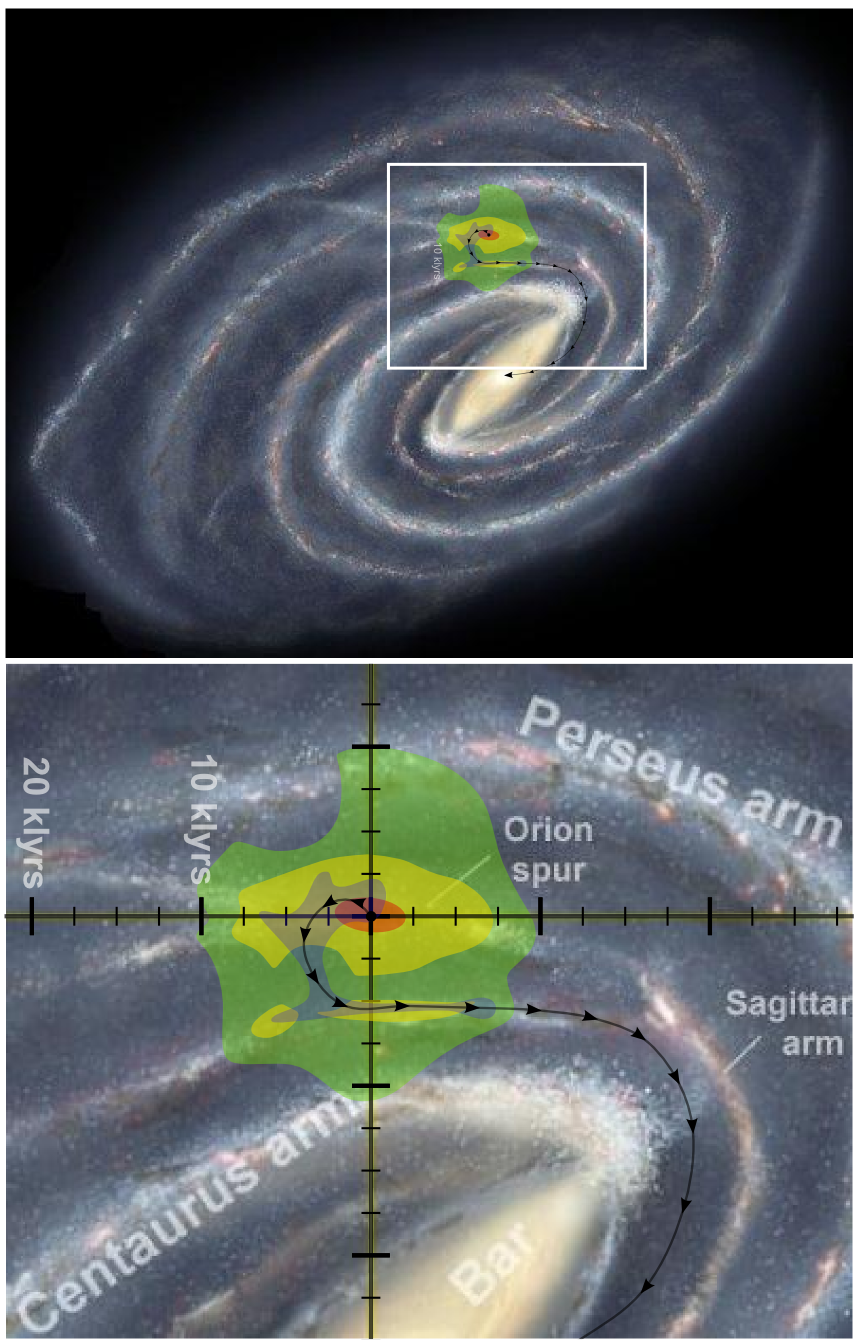
\includegraphics[width=0.75\textwidth]{map.png}
\caption{Karte der Milchstraße mit Heimat (Orange), Grenzland (Gelb) und Wildnis (Grün). Außerdem ist der Kreuzzug Urbans des XXIV als größte interstellare Bewegung eingezeichnet.}
\end{figure}

\section{Klassifikation - Planeten}
\begin{itemize}
\item \textbf{Tot:} atmosphärelos oder giftige Atmösphäre, unfruchtbar für jede Form von Leben (Merkur, Venus...)
\item \textbf{Urzeitlich:} flüssiges Wasser, kurzzeitig atembare Atmosphäre, mikrobielles Leben, einfache Algen. Evtl. aktive Terraformer anwesend.
\item \textbf{Wild:} Höheres nichtintelligentes Leben (vgl. Erdmittelalter). Langfristige Kolonisation möglich, aber (noch?) nicht geschehen.
\item \textbf{Fehlschlag:} Fehlfunktion der Saatschiff-KIs mit verstörenden, erstaunlichen oder unfassbaren folgen. Schwer in obiges Schema  einzuordnen.
\item \textbf{Kolonie:} Langfristig stabile menschliche Population anwesend. Siehe Zivilisationsstufen.
\end{itemize}

\section{Klassifikation - Zivilisationen}
\begin{itemize}
\item \textbf{Archaisch (Stufe 0):} Menschlich besiedelt, Rückfall in einfachste Stammesstrukturen, Jäger- und Sammlergesellschaften. Meist stark religiöse/ritualistische Strukturen (vgl. Azteken, Massai, mongolische Nomadenstämme...) Gelegentliche Nutzung technologischer Artefakte ohne eigentliches Verständnis.
\item \textbf{Mittelalterlich (Stufe I):} Dichter besiedelt mit Stadtentwicklung, häufig monarchische, demokratische oder theokratische Gesellschaften (vgl. Römisches Reich, feudales Japan, Europäisches Mittelalter). Teilweise breitere Nutzung und Handel mit unverstandenen Hochtechnologien (häufig Aufgabe einer Magotechnischen oder Priesterlichen Kaste).
\item \textbf{Modern (Stufe II):} Globalisierte Zivilisation mit massivem Eingriff in die planetare Entwicklung (vgl. heutige Erde). Grundlegende Raumfahrt im nahen Orbit, Kenntnis von der Vorgeschichte der Menschheit. Fähigkeit zur Nutzung und Verständnis auch überlegener Technologien.
\item \textbf{Post-Kollaps:} Moderne Zivilisation nach globaler Katastrophe: Kollaps des Ökosystems, Asteroideneinschlag, Thermonuklearer Krieg oder Zerstörung durch Kräfte von außen (vgl. Erde ,,nach dem 3. Weltkrieg''). Leben zwischen Ruinen mit Erinnerungen an ,,die Zeit davor''. Allmählicher Übergang in mittelalterliches oder archaisches Stadium.
\item \textbf{Interplanetar (Stufe III):} Weitläufige Besiedlung des Sternensystems mit aktiver interplanetarer Raumfahrt. Möglicherweise Bau neuer Sternenschiffe (vgl. Erde vor dem Aufbruch)
\item \textbf{Transzendent (Stufe IV):} Systeme nach der technologischen Singularität, beherrscht von Maschinengöttern oder posthumanen Wesenheiten. Von menschlicher Intelligenz weder zu begreifen noch zu beeinflussen.
\end{itemize}

\chapter{Die Menschheit}
\section{Rassen}
Durch genetische Modifikationen und extreme Umwelt\-bedin\-gungen hat die menschliche Evolution einige stark abweichende Seitenlinien hervorgebracht. Die meisten der folgenden Rassen sind natürlich vorwiegend in ent\-sprechend hochtechnisierten Kulturen entstanden, da die modifizierten Gene jedoch teilweise vererbt werden lassen sich auch auf niedrig entwickelten Planeten Abstammungslinien mit diesen Eigenschaften finden (die dann oft als Hexen verfolgt oder als Halbgötter angebetet werden...).

\begin{figure}[h!]
\subsection*{Homo Sapiens:} Immer noch der am weitesten verbreitete Menschentypus.
\begin{itemize}
\item \textbf{Anpassungsfähig:} Ein freies Talent bei der Generierung
\end{itemize}
\end{figure}

\begin{figure}[h!]
\subsection*{Himmelsgeborene:} Menschen die den Großteil ihres Lebens im All verbringen entwickeln deutlich überlegene räumliche Wahrnehmung und Koordinationsvermögen. Der Muskelschwund lässt sich aber auch mit modernster Medizin nicht vollkommen aufhalten.
\begin{itemize}
\item \textbf{Anpassungsfähig:} Ein freies Anfänger-Talent bei der Generierung
\item \textbf{Muskelschwund:} Stärke wird während der Generierung zu doppelten Kosten gesteigert.
\item \textbf{3D-Bewegung:} Beginnt mit d6 auf Geschicklichkeit.
\end{itemize}
\end{figure}

\begin{figure}[h!]
\subsection*{Zwerg:} Menschen die auf Planeten mit mehr als der doppelten Erdschwerkraft aufwachsen entwickeln eine gedrungene, stämmige Gestalt. Für die meisten normalen Menschen ist ein dauerhaftes Leben unter solchen Bedingungen kaum vorstellbar.
\begin{itemize}
\item \textbf{Anpassungsfähig:} Ein freies Anfänger-Talent bei der Generierung
\item \textbf{Kräftig gebaut:} Beginnt mit d6 auf Stärke.
\item \textbf{Kurze Beine:} Geschwindigkeit 4 (nur d4 Sprint).
\end{itemize}
\end{figure}

\begin{figure}[h!]
\subsection*{Narziss:} Auf wohlhabenderen High-Tech-Welten sind perfektionierte Designer-Kinder keine Seltenheit. Die meisten Schönheitsideale stellen Widerstandskraft gegen Gewalteinwirkung aber eher hinten an.
\begin{itemize}
\item \textbf{Anpassungsfähig:} Ein freies Anfänger-Talent bei der Generierung
\item \textbf{Vollendetes Design:} +2 Charisma
\item \textbf{zerbrechliche Schönheit:} -1 Robustheit.
\end{itemize}
\end{figure}

\begin{figure}[h!]
\subsection*{Ghul:} Überbegriff für Menschen, die gutartige, aber scheußlich anzusehende Fehlbildungen durch Umweltgifte oder Strahlung erlitten haben (hier hilft auch aufwändigste plastische Chirurgie kaum weiter). Aufgrund ihres Aussehens sind ihnen viele Wege verbaut, die meisten entwickeln sich daher zu verbissenen Einzelkämpfern.
\begin{itemize}
\item \textbf{Entstellt:} -2 Charisma.
\item \textbf{Furchteinflößend:} Beginnt mit d6 auf Einschüchtern.
\item \textbf{Abgehärtet:} Beginnt mit d6 auf Willenskraft.
\end{itemize}
\end{figure}

\begin{figure}[h!]
\subsection*{Gray:} Menschen, denen vor der Geburt auf biotechnischem Weg der Alterungsprozess deaktiviert wurde (Stichwort: Telomerase). Dies bringt jedoch nicht nur Vorteile mit sich...
\begin{itemize}
\item \textbf{Alterslos:} Die Lebenszeit ist ohne äußere Einwirkungen unbegrenzt.
\item \textbf{Im Angesicht der Ewigkeit:} Beginnt mit einer schweren Geistesstörung nach Wahl (z. B. Suizidwunsch/Unachtsamkeit, Phobie vor Einsamkeit/Leeren Räumen/dem All).
\item \textbf{Geduldig:} Beginnt mit d6 auf Verstand.
\end{itemize}
\end{figure}

\begin{figure}[h!]
\subsection*{Spartiat/Walküre:} Im Krieg endet jegliche Moral. Auf den meisten Welten auf denen dies technisch möglich ist werden genetisch überzüchtete Supersoldaten mit übermenschlichen Reflexen erschaffen und das  kritische Denkvermögen aberzogen.
\begin{itemize}
\item \textbf{Übermensch:} Beginnt mit d8 auf Geschicklichkeit und darf diesen Wert mit gewöhnlichen Steigerungen bis auf d12+2 bringen.
\item \textbf{Redundante Organe:} +2 auf alle Würfe um widrigen Umweltbedingungen (Kälte, Hitze, Strahlung, Vakuum...) zu widerstehen.
\item \textbf{Konditioniert:} Wenn sie von einer gerechtfertigten Position kommen (Respektspersonen, Freunde) werden Befehle ausgeführt ohne sie zu hinterfragen.
\item \textbf{verkümmerte Abstraktionsfähigkeit} -1 auf Wissensproben die keinen direkten Bezug zur Kriegsfühurung haben.
\end{itemize}
\end{figure}

\begin{figure}[h!]
\subsection*{Kind der Maschine:} Der Charakter ist auf einer Welt groß geworden auf der Körpermodifikationen weithin akzeptiert sind. Er beginnt bereits mit einem stark vercyberten Körper und hat weniger Probleme mit Abstoßungsreaktionen und Entfremdung.
\begin{itemize}
\item \textbf{Eins mit der Maschine:} Das Cyberware-Limit ist generell um 2 Punkte erhöht.
\item \textbf{Verbessert:} Der Charakter beginnt mit entweder zwei Teilen Cyberware der Klasse I, einem Teil der Klasse II oder einer zusätzlichen Gliedmaße (Klasse II).
\item \textbf{Anfällige Technik:} -4 Auf Würfe gegen Strahlungseinflüsse und EMP.
\item \textbf{Fremdartig:} -2 Charisma bei Begegnungen mit nicht vercyberten Menschen.
\end{itemize}
\end{figure}

\section{Kulturen}
\subsection*{Die Hegemonie}
Eine der wenigen tatsächlich stabilen interstellaren Zivilisationen und wohl eine der fortschrittlichsten Gesellschaften die die Menschheit hervorbrachte. Die meisten Planeten der Hegemonie beherbergen postmaterielle Gesellschaften, ihre Bewohner hängen einer sehr freiheitlichen, hedonistischen Ideologie an. Dennoch sieht die Hegemonie ihren Wohlstand als Verantwortung an, diesen auch dem Rest der Menschheit zu bringen. In interstellaren Feldzügen werden autoritäre Regierungen gestürzt, und primitiven Gesellschaften das ,,Geschenk der Technologie'' gebracht. Dabei ist die Hegemonie aber stehts auf innere Stabilität bedacht, weshalb Flüchtlinge von außen mit eiserner Hand abgewiesen werden.\\
Ihren Wohlstand verdankt die Hegemonie dem freien Fluss von Information, Wissen und Kulturgütern zwischen ihren Systemen, und der aufs strengste kontrollierten Balance zwischen High-Tech-Produktionsmitteln und einer über strenge Geburtenkontrolle stabil gehaltenen Bevölkerung.\\
(Kurzfassung: Interstellares Technokratisches Utopia mit starkem Sendungsbewusstsein.)
\begin{itemize}
\item Spartiaten sind als Rasse ungeeignet, da sich ein solcher Missbrauch einer menschlichen Existenz hier moralisch völlig verbietet.
\end{itemize}
\subsection*{Die sterbende Sonne}
So viele Spekulationen, Sagen und Legenden ranken sich um die alte Heimat der Menschheit, das sich niemand zu sagen vermag, was man heutzutage dort vorfinden würde. Gelegentlich werden Sonden oder wagemutige Abenteurer auf Erkundungsmission geschickt... um letztlich nie wiedergefunden zu werden. Die verlässlichsten Daten sind bei den Sehern zu finden: bizarr deformierte Planeten- und Sonnenspektren, für die selbst die erfahrendsten unter ihnen keine Erklärung geben können. Letztlich können auch sie nur spekulieren, was die alte Menschheit ausgelöscht (oder entrückt?) hat. Grandios fehlgeschlagene planetare und stellare Manipulationen? Hat die Menschheit eine Form von Transzendenz erlangt und sich bewusst vom Rest des Universums abge\-schottet? Oder hat sie den Zorn noch mächtigerer Wesenheiten auf sich gezogen?

\subsection*{Die aufgehende Sonne}
Moderne hoch computerisierte und vernetzte Gesellschaft, die versuchen eine Balance zwischen Spiritualität und Technik zu finden. Die am weitesten verbreitete Religion ist eine fortgeschrittene Form des Shinto-Buddhismus. Zentrale Bedeutung hat ein Cyberspace-Ahnenkult: Verstorbene hinterlassen einen Avatar voller Erinnerungen und Erfahrungen, der weiterhin sein ,,Leben'' mit den Hinterbliebenen teilt und von diesen respektiert und um Rat ersucht wird. Auch in anderen Bereichen ist der Umgang mit Technologie nicht immer von Rationalität geprägt und die Vorstellung von Geistern in der Maschine ist weit verbreitet.\\

Die einzelnen Welten der aufgehenden Sonne sind politisch weitgehend voneinander unabhängig und die Technosphären ihrer Planeten durch die Jahrelangen Kommunikationsverzögerungen zwischen den Sternen getrennt. Die konservative und stabile Kultur sorgt dennoch dafür, dass die Kulturen der einzelnen Welten sich stark ähneln.
(Kurzfassung: Klassische Cyberpunk-Welten geprägt von fernöstlicher Mystik.)
\begin{itemize}
\item Sehr verbreitet sind Kinder der Maschine, verbotene Rassen gibt es keine.
\end{itemize}

\subsection*{Das Reich der 1000 Pharaonen}
Die Ursprünge des Reiches sind im Dunkel der Geschichte verlorengegangen; bekannt ist, dass heute jedem System des Reiches ein vergöttlichter, unsterblicher (siehe: Gray) Pharao vorsteht, die offenbar allesamt Klone ein- und derselben Person sind, und meist eine gemeinsame Agenda verfolgen. Über die exakte Zahl der Pharaonen und ob bzw. wo der ursprüngliche lebt ist nichts bekannt. Die regierungsweise ist hierarchisch und autoritär, die Interessen des Pharaos werden von einer Magotechnischen Priesterkaste durchgesetzt während ein Großteil der Bevölkerung auf technisch niedrigem (aber nicht zwangsläufig armem) Niveau gehalten wird. Die Pharaonen schaffen es jedoch die Arbeitskraft ihrer Bevölkerung in atemberaubende Großprojekte zu kanalisieren, die auch die anderen Zentralwelten in Staunen versetzen.\\
(Kurzfassung: Theokratisches Großreich, zusammengehalten von einem visionären Herrscher und dem Stolz eines Volkes auf seine Schaffenskraft)
\begin{itemize}
\item Die Unsterblichkeit ist dem Pharao vorbehalten. Grays werden verfolgt und beseitigt und sind entsprechend als Rasse ungeeignet.
\item Kinder der Maschine sind nur in der Priesterkaste, nicht jedoch in der niederen Bevölkerung anzutreffen. 
\end{itemize}

\subsection*{Urbans letzter Kreuzzug}
Vor Jahrhunderten rief der prophetische Papst Urban XXIV die verstreuten Überbleibsel des Christentums zum Exodus in Richtung des Galaktischen Zentrums auf, wo nach seiner Vision der Menschheit der Sinn des Universums offenbart werden soll. Seit sich die Nachricht durch die besiedelten Gebiete verbreitete sammeln sich zahllose Generationen- und Schläferschiffe zur größten je dagewesenen Flotte, die langsam durch die Randwelten zieht. Der Kreuzzug ist nicht offen kriegerisch, jedoch kann schon die Durchreise der Flotte wie auch die Missionierungsversuche in rückstandigeren Systemen einen extremen Kulturschock verursachen der gelegentlich auch gewaltsam eskaliert.\\
(Kurzfassung: Streng gläubiges raumfahrendes Volk auf der letzten großen Mission der Menschheit.)
\begin{itemize}
\item Da der Mensch nach dem Ebenbild Gottes geschaffen wurde, gilt eine ,,Verbesserung'' durch Cyberware als anmaßend und ketzerisch. Kinder der Maschine sind hier nicht anzutreffen.
\item Ein Großteil der Kreuzfahrer verbringt sein gesamtes Leben auf einem Sternenschiff. Himmelsgeborene sind daher als Rasse weit verbreitet.
\end{itemize}

\subsection*{Einherjer}
Benannt von Außenstehenden nach dem Einsatz ihrer Schiffsgeschütze, der einen wilden und gnadenlosen Angriff einleitet, und den meisten eher wie eine Naturgewalt erscheint. Selbst bezeichnen sie sich jedoch als Einherjer. Das kriegerische, neo-paganistische Volk ist höchstwahrscheinlich aus der Sternenflotte eines längst untergegangenen Reiches hervorgegangen; heute haben sie sich weit über die Grenzen der bewohnbaren Gebiete verteilt. Als berüchtigte Entdecker verbreiten sie nicht nur Angst und Schrecken in den Randwelten, sondern schieben auch die Grenzen der bekannten Welt immer weiter voran, wobei sie in einer Mischung aus Furcht und Verehrung den Spuren der Wanen folgen, die das Leben über die Galaxis säen. Die Plünderungen bewohnter Planeten erfolgen dabei nicht aus wahlloser Brutalität, sondern sind eine reine Notwendigkeit zum Überleben in der rauhen Wildnis.\\
(Kurzfassung: Sternenfahrendes Volk von wagemutigen Entdeckern und gefürchteten Kriegern ohne zentrale Organisation.)
\begin{itemize}
\item Auf so gut wie jedem Schiff findet sich eine schlagkräftige Truppe von Walküren, die die Angriffe führen.
\item Bei dem raumfahrenden Volk sind Himmelsgeborene weit verbreitet.
\item Einige Schiffe haben Seher der Leere an Bord, die hier unter dem Namen der Nornen auch eine mystische Funktion innehaben.
\end{itemize}

\subsection*{Die Seher der Leere}
\textit{,,Wie Plankton treiben wir durch diesen kosmischen Sturm aus Licht und Gravitation, unsere Lebensspannen so kurz, unsere Horizonte so winzig, dass wir nicht einmal wahrnehmen, wie die Wellenberge sich über uns auftürmen.''}\\ - Antwort der Seher auf die Frage nach dem Platz des Menschen im Kosmos\\	\

Die Seher der Leere horten ihre Geheimnisse in Akademien, die sich auf toten Planeten und Raumstationen im Orbit um das dutzend Pulsare finden, die weithin nur ,,Leuchttürme'' genannt werden. Hier finden sich angeblich Datenbanken in denen jeder einzelne Stern und Planet der Milchstraße verzeichnet sind und die Seher sollen nicht nur einen Großteil dieser Daten in ihrer Erinnerung (oder in Implantaten?) tragen sondern auch das komplette bis dahin bekannte physikalische Modell. Dieses Wissen macht sie zu unübertroffenen Navigatoren und Wissenschaftlern, ihre extrem nihilistischen Sichtweisen auf die Bedeutung der Menschheit machen jedoch den Umgang mit ihnen äußerst befremdlich.\\
(Kurzfassung: Eigenbrötlerische Hüter von unschätzbarem Wissen und finstere Mystiker)
\begin{itemize}
\item allein die Grundausbildung zum Seher übersteigt die Lebenszeit eines gewöhnlichen Menschen, auf den Akademien sind daher ausschließlich Gray anzutreffen.
\end{itemize}

\subsection*{Der Kataklysmus}
Eine Hypernova sterilisierte ein Gebiet von einigen Lichtjahren um den Vorgängerstern. Verheerendere Auswirkungen hatte jedoch der elektromagnetische und Teilchensturm, der noch weit über diesen Bereich von einer Sekunde auf die andere jegliche elektronische Technologie zerstörte, und damit zum Kollaps eines ganzen Sektors in die mittelalterliche Technologiestufe führte.
\begin{itemize}
\item Kinder der Maschine sind hier natürlich nicht mehr zu finden.
\item In den Ruinen der Vorgängerzivilisationen sind häufig Ghule anzutreffen.
\end{itemize}

\subsection*{Das Bollwerk}
\subsection*{Die Fehlfunktion}

\chapter{Mystik}
Ein Großteil des Legendenschatzes der alten Menschheit hat in Datenbanken und Erzählungen überlebt. Gerade in den Grenzgebieten spielen diese eine wichtige Rolle im Leben der Menschen. Längst vergessene Gottheiten werden wieder verehrt, ganze Gesellschaften werden (teilweise romantisch verklärten...) Vorbildern von der alten Erde nachempfunden, weshalb viele Systeme, Planeten und Sternenschiffe Namen tragen die dort ihren Ursprung nahmen. Auch streng religiöse raumfahrende Völker kommen vor.

\section{Monolithen und Megalithen}
Wann der erste Monolith entdeckt wurde ist unbekannt, Fakt ist dass sie offenbar ein weit verbreitetes Phänomen in der Galaxis sind. Ein Großteil der bewohnbaren Planeten beherbergen wenige dutzend bis hundert über den Planeten verteilte Monolithen, meist zusammen mit einer deutlich größeren Ausgabe, dem Megalithen. Megalithen bilden meist einen Kondensationspunkt für die kulturelle, religiöse und wissenschaftliche Entwicklung eines Planeten und werden Zentren von Pilgerstätten und Forschungseinrichtungen, aber auch Streitobjekt selbst interplanetarer Kriege. Herkunftserklärungen über die Monolithen finden sich im Kern vieler Religionen, aber auch wissenschaftlicher Theorien, die das Phänomen jedoch nicht einmal in Ansätzen fassen können.\\
Ob es sich nun um die Hinterlassenschaften außerirdischer ,,Erstgeborener'', Geschenke Gottes an die Menschheit oder auf natürlichem Weg  kristallisierte exotische Materie handelt, die Monolithen beherbergen eine Macht, die zwar von Menschen genutzt, aber wohl nie vollends verstanden werden kann.\\

\newpage
\section{Arkane Hintergründe}
Alle Formen übernatürlichen Wirkens sind mehr oder weniger direkt an die Monolithen gekoppelt. Gemein ist, dass die meisten Arkanen mindestens einmal im Leben (nicht zwangsläufig bewusst) mit einem Megalithen in Kontakt gekommen sein müssen (häufig Teil eines Initiationsritus).\\ Regeltechnisch werden übernatürliche Fähigkeiten über die Talente Wunderwirken, Psi-Kräfte und Grenzwissenschaft abgehandelt, die gleichzeitig auch die Interpretation der Fähigkeiten darstellen. Dementsprechend schließen sich die drei Fähigkeiten gegenseitig aus.\\
Die Spezialisierungen der Talente entsprechen einer engeren Denkschule und kommen mit einem eingeschränkten Satz an erlernbaren Fertigkeiten. Jeder Machtwirker beginnt mit einer Spezialisierung und ist an deren Grenzen gebunden. Ein Ausbrechen aus dieser Denkschule ist prinzipiell möglich, aber häufig durch Doktrinen oder Glaubensgrundsätze gehemmt.
\begin{itemize}
\item \textbf{Wunder:} v. a. Tech 0 und I Planeten. Viele Kulturen sehen die Macht der Monolithen als Gabe von Göttern oder Naturgeistern an. Wunderwirkende sind häufig an starke kulturell verwurzelte Prinzipien gebunden; Brechen dieser Prinzipien führt zu starken Selbstzweifeln oder einer unterschwelligen Furcht vor der Missgunst des Gottes und macht das Einsetzen der Macht über mittellange Zeiträume unmöglich.
\begin{itemize}
\item Priestertum
\item Druidentum
\item Voodoo
\end{itemize}
\item \textbf{Psi-Kräfte:} v. a. Tech I bis III Planeten. Einige Philosophien glauben an Mächte die den Menschen selbst oder der Natur innewohnen und nur von diesen entfesselt werden müssen, unabhängig von einer personifizierten, übernatürlichen Macht. Ihnen gemein ist, das beim Überschreiten der Fähigkeiten die Gefahr eines schädlichen Kontrollverlustes besteht.
\begin{itemize}
\item Magie
\item Zen-Mystik
\item Psionik
\end{itemize}
\item \textbf{Grenzwissenschaften:} v. a. Tech II bis III Planeten. Hierunter werden Machtwirker zusammengefasst, die Technologien einsetzen, die sie nicht vollends verstehen. Sie gehen davon aus, dass ihre Fähigkeiten in einem fortschrittlicheren Weltbild wissenschaftlich erklärbar wären. Es besteht jedoch immer die Gefahr, dass die Gerätschaften verheerenden Fehlfunktionen unterliegen.
\begin{itemize}
\item Grand Unified Theory
\item Nanoschwärme
\item Symbiotik
\item Mindhacking
\end{itemize}
\end{itemize}

\onecolumn
\chapter{Eine Savage Worlds Implementierung}
Die Setting-Sonderregeln zur Talentspezialisierung und zu dauerhaften Wunden (Gritty Damage) werden genutzt, und die Initiative wird über einen W12 ermittelt.

\section{Rassen}
\begin{figure}[h!]
\subsection*{Homo Sapiens:} Immer noch der am weitesten verbreitete Menschentypus.
\begin{itemize}
\item \textbf{Anpassungsfähig:} Ein freies Talent bei der Generierung
\end{itemize}
\end{figure}

\begin{figure}[h!]
\subsection*{Himmelsgeborene:}
\begin{itemize}
\item \textbf{Anpassungsfähig:} Ein freies Anfänger-Talent bei der Generierung
\item \textbf{Muskelschwund:} Stärke wird während der Generierung zu doppelten Kosten gesteigert.
\item \textbf{3D-Bewegung:} Beginnt mit d6 auf Geschicklichkeit.
\end{itemize}
\end{figure}

\begin{figure}[h!]
\subsection*{Zwerg:}
\begin{itemize}
\item \textbf{Anpassungsfähig:} Ein freies Anfänger-Talent bei der Generierung
\item \textbf{Kräftig gebaut:} Beginnt mit d6 auf Stärke.
\item \textbf{Kurze Beine:} Geschwindigkeit 4 (nur d4 Sprint).
\end{itemize}
\end{figure}

\begin{figure}[h!]
\subsection*{Narziss:}
\begin{itemize}
\item \textbf{Anpassungsfähig:} Ein freies Anfänger-Talent bei der Generierung
\item \textbf{Vollendetes Design:} +2 Charisma
\item \textbf{zerbrechliche Schönheit:} -1 Robustheit.
\end{itemize}
\end{figure}

\begin{figure}[h!]
\subsection*{Ghul:}
\begin{itemize}
\item \textbf{Entstellt:} -2 Charisma.
\item \textbf{Furchteinflößend:} Beginnt mit d6 auf Einschüchtern.
\item \textbf{Abgehärtet:} Beginnt mit d6 auf Willenskraft.
\end{itemize}
\end{figure}

\begin{figure}[h!]
\subsection*{Gray:}
\begin{itemize}
\item \textbf{Alterslos:} Die Lebenszeit ist ohne äußere Einwirkungen unbegrenzt.
\item \textbf{Im Angesicht der Ewigkeit:} Beginnt mit einer schweren Geistesstörung nach Wahl (z. B. Suizidwunsch/Unachtsamkeit, Phobie vor Einsamkeit/Leeren Räumen/dem All).
\item \textbf{Geduldig:} Beginnt mit d6 auf Verstand.
\end{itemize}
\end{figure}

\begin{figure}[h!]
\subsection*{Spartiat/Walküre:}
\begin{itemize}
\item \textbf{Übermensch:} Beginnt mit d8 auf Geschicklichkeit und darf diesen Wert mit gewöhnlichen Steigerungen bis auf d12+2 bringen.
\item \textbf{Redundante Organe:} +2 auf alle Würfe um widrigen Umweltbedingungen (Kälte, Hitze, Strahlung, Vakuum...) zu widerstehen.
\item \textbf{Konditioniert:} Wenn sie von einer gerechtfertigten Position kommen (Respektspersonen, Freunde) werden Befehle ausgeführt ohne sie zu hinterfragen.
\item \textbf{verkümmerte Abstraktionsfähigkeit} -1 auf Wissensproben die keinen direkten Bezug zur Kriegsfühurung haben.
\end{itemize}
\end{figure}

\begin{figure}[h!]
\subsection*{Kind der Maschine:}
\begin{itemize}
\item \textbf{Eins mit der Maschine:} Das Cyberware-Limit ist generell um 2 Punkte erhöht.
\item \textbf{Verbessert:} Der Charakter beginnt mit entweder zwei Teilen Cyberware der Klasse I, einem Teil der Klasse II oder einer zusätzlichen Gliedmaße (Klasse II).
\item \textbf{Anfällige Technik:} -4 Auf Würfe gegen Strahlungseinflüsse und EMP.
\item \textbf{Fremdartig:} -2 Charisma bei Begegnungen mit nicht vercyberten Menschen.
\end{itemize}
\end{figure}


\section{Fertigkeitsbaum}
\begin{figure}[h!]
\center
\includegraphics[scale=0.47]{skills.png}
\end{figure}

\section{Talente}


\section{Waffentechnik}
\subsection*{Rüstungen}

\begin{table}
\begin{tabular}{|c|c|c|c|c|c|}
\hline 
\textbf{Rüstungen} & Tech & Panzerung & Gewicht & Kosten & Anmerkungen \\ 
\hline 
Lederrüstung & 0 & +1 & 15 & 50 & Torso, Arme, Beine \\ 
\hline 
Kettenhemd & I & +2 & 25 & 300 & T, A, B \\
\hline 
Platte (voll) & I & +3 & 50 & 900 & T, A, B \\
\hline 
Gewebe & II & +1 & 2 & 100 & T, A, B \\ 
\hline 
Kevlarweste & II & +2/+4* & 8 & 250 & T, *nur gg. Kugeln \\
\hline 
Kevlar/Keramik & II & +4/+8* & 12 & 2500 & T, *nur gg. Kugeln \\ 
\hline 
Infanterieanzug & II & +6 & 20 & - & Ganz \\ 
\hline 
Panzeranzug & II & +8 & 30 & - & G \\ 
\hline 
Reflektive Weste & III & -/+10* & 5 & 200 & T, *nur gg. Laser \\ 
\hline 
Exo: Späher & III & +10 & 0 & - & G, aktive Camouflage \\ 
\hline 
Exo: Kampf & III & +12 & 0 & - & G, unterstützend \\ 
\hline 
Exo: Schwer & III & +14 & 0 & - & G, langsam, schwere Waffe \\
\hline 
\textbf{Helme}\\ 
\hline
Lederhelm & 0 & +1 & 3 & 10 & Kopf, 50\% der Treffer \\
\hline 
Topfhelm & I & +2 & 4 & 60 & K, 50\% \\
\hline
Motoradhelm & II & +3 & 5 & 75 & K, 50\% \\
\hline 
Stahlhelm & II & +4 & 5 & 80 & K, 50\% \\
\hline 
\textbf{Schilde}\\ 
\hline 
Holzschild & 0 & -/+1* & 8 & 25 & Parade +1, *nur gg. FK \\ 
\hline 
Bronzeschild & I & -/+2* & 12 & 50 & Parade +1, *nur gg. FK \\ 
\hline 
Turmschild & I & -/+2* & 20 & 200 & Parade +2, *nur gg. FK \\ 
\hline 
Riot Shield & II & -/+3* & 15 & - & Parade +2, *nur gg. FK \\ 
\hline 
Ballist. Schild & II & -/+4* & 30 & - & Parade +2, *nur gg. FK \\ 
\hline 
\end{tabular} 
\end{table}


\subsection*{Nahkampfwaffen}
\begin{table}
\begin{tabular}{|c|c|c|c|c|c|}
\hline 
\textbf{Kurzwaffen} & Tech & Schaden & Gewicht & Kosten & Anmerkungen \\ 
\hline 
Faustkeil & 0 & Stä+W4-2 & 3 & 1 &  \\ 
\hline 
Steinbeil & 0 & Stä+W4-1 & 4 & 5 &  \\
\hline 
Dolch & 0 & Stä+W4 & 1 & 25 &  \\
\hline 
Handaxt & I & Stä+W6 & 2 & 200 &  \\ 
\hline 
Kurzschwert & I & Stä+W6 & 4 & 200 &  \\ 
\hline 
Schlagstock & II & Stä+W4 & 1 & 10 & \\ 
\hline 
Schnappmesser & II & Stä+W4 & 1 & 20 & -2 auf Durchsuchungstests \\
\hline 
Schweißbrenner & II & 2W6 & 10 & 200 & Sekundäreffekt: Feuer \\ 
\hline 
Shockstick & II & Stä+W6 & 2 & - & nichtletaler Schaden \\ 
\hline 
Molekularmesser & III & Stä+W4+2 & 1 & - & PB\,2 \\ 
\hline 
\end{tabular}
\end{table}

\begin{table}
\begin{tabular}{|c|c|c|c|c|c|}
\hline 
\textbf{Mittellang} & Tech & Schaden & Gewicht & Kosten & Anmerkungen \\ 
\hline 
Langschwert & I & Stä+W8 & 8 & 300 &  \\ 
\hline 
Rapier & I & Stä+W4 & 3 & 150 & Parade\,+1 \\
\hline 
Katana & I & Stä+W6+2 & 6 & 1000 & PB\,2 \\
\hline 
Zweihänder & I & Stä+W10 & 12 & 400 & Parade\,-1, 2H \\ 
\hline 
Streithammer & I & Stä+W6 & 8 & 250 & PB\,1 \\ 
\hline 
Streitaxt & I & Stä+W8 & 10 & 300 & \\ 
\hline 
2H-Axt & I & Stä+W10 & 15 & 500 & PB\,1, Parade\,-1, 2H \\
\hline 
2H-Hammer & I & Stä+W8 & 20 & 400 & PB\,1, Parade\,-1, 2H \\ 
\hline 
Kettensäge & II & 2W+4 & 20 & 200 & Eigentreffergefahr \\ 
\hline 
Bangstick & II & 3W6 & 2 & 5 & Nachladen: 1\,Akt. \\ 
\hline 
Mol. Schwert & III & Stä+W8+2 & 1 & 500 & PB\,4 \\ 
\hline 
\end{tabular}
\end{table}

\begin{table}
\begin{tabular}{|c|c|c|c|c|c|}
\hline 
\textbf{Stabwaffen} & Tech & Schaden & Gewicht & Kosten & Anmerkungen \\ 
\hline 
Kampfstab & 0 & Stä+W4 & 8 & 10 & Parade\,+1, 2H \\
\hline
Speer & 0 & Stä+W6 & 5 & 100 & Parade\,+1, 2H \\ 
\hline 
Hellebarde & I & Stä+W8 & 15 & 250 & 2H \\
\hline 
Reiterlanze & I & Stä+W8 & 10 & 300 & PB\,2, nur vom Pferd \\ 
\hline 
Pike & I & Stä+W8 & 25 & 400 & 2H, lang \\ 
\hline 
Bajonett & II & Stä+W6 & 1 & 25 & Parade\,+1, 2H \\ 
\hline 
Schocklanze & II & Stä+W8 & 10 & - & nichtlethaler Schaden \\ 
\hline 
Mol. Lanze & III & Stä+W8+2 & 15 & - & PB\,6, 2H \\ 
\hline 
\end{tabular} 
\end{table}


\subsection*{Fernkampfwaffen}
\begin{table}
\begin{tabular}{|c|c|c|c|c|c|c|c|}
\hline 
\textbf{Wurfwaffen} & Tech & Reichweite & Schaden &  Kosten & Gew & Stä & Anmerkungen \\ 
\hline 
Stein & 0 & 3/6/12 & Stä+W4-2 & 0 & 1 & - &  \\ 
\hline 
Schleuder & 0 & 4/8/16 & Stä+W4 & 10 & 1 & - &  \\ 
\hline 
Dolch & 0 & 3/6/12 & Stä+W4 & 25 & 1 & - &  \\ 
\hline 
Speer & 0 & 3/6/12 & Stä+W6 & 100 & 5 & W6 & \\ 
\hline 
Netz/Bola & 0 & 3/6/12 & -* & 10 & 5/2 & - & *Einfangen \\ 
\hline 
Beil & I & 3/6/12 & Stä+W6 & 75 & 2 & - & \\ 
\hline 
Sprengsätze & & 4/8/16 & & - & 4 & - & \\ 
Dynamit & I & Mittel & 2W6 & & & & \\
Granate & II & Mittel & 3W6 & & & & \\
Pionier-Ldg. & II & Groß & 4W6 & & & W6 & \\
Flash & II & Mittel & -* & & & & *Blenden \\
EMP & III & Mittel & -* & & & & *Schock \\
Koffer-Nuke & III & Groß & 3W10* & & & W6 & *Strahlung\\
\hline 
Filamentbola\ & III & 3/6/12 & Stä+W4+2* & - & 2 & - & PB\,2, *Einf. \\ 
Schockbola & II & & Stä+W4* & & & - & *nichtlethal, Einf. \\ 
\hline
\end{tabular}
\end{table}

\begin{table}
\begin{tabular}{|c|c|c|c|c|c|c|c|}
\hline 
\textbf{Mech. Waffen} & Tech & Reichweite & Schaden &  Kosten & Gew & Stä & Anmerkungen \\ 
\hline 
Bogen & 0 & 12/24/48 & 2W6 & 200 & 3 & W6 &  \\ 
\hline 
Langbogen & I & 15/30/60 & 2W6 & 250 & 5 & W8 &  \\ 
\hline 
Armbrust & I & 15/30/60 & 2W6 & 500 & 10 & W6 & PB\,2, NL 1\,Akt. \\ 
\hline 
Compoundbogen & II & 15/30/60 & & 500 & 5 & W6 & \\ 
Standardpfeil & II & - & 2W8 & & & & \\
Sprengpfeil & II & klein & 3W6 & & & & \\
Blendpfeil & II & Mittel & -* & & & & *Blenden \\
EMP-Pfeil & III & klein & -* & & & & *Schock \\
\hline 
Compoundarmbrust & II & 24/48/96 & 2W8 & 1000 & 8 & W6 & PB\,2, NL 1\,Akt. \\ 
\hline
Repetierarmbrust & II & 15/30/60 & 2W6 & - & 10 & - & PB\,2, 6 Schuss \\ 
 & & & & & & & dann NL 1\,Akt. \\
\hline
\end{tabular}
\end{table}

\begin{table}
\begin{tabular}{|c|c|c|c|c|c|c|c|c|}
\hline 
\textbf{Feuerwaffen} & Tech & Reichweite & Schaden & FR & Kosten & Gew & Schuss & Anmerkungen \\ 
\hline 
Muskete 	& I & 10/20/40 & 2W8 & 1 & 200 & 12 & 1 & NL 2\,Akt. \\ 
\hline 
Steinschloss- & I & 5/10/20 & 2W6+1 & 1 & 250 & 3 & 1 & NL 2\,Akt. \\ 
pistole & & & & & & & & \\
\hline 
Colt 	& II & 12/24/48 & 2W6+1 & 1 & 200 & 4 & 6 & Revolver \\ 
\hline 
D. Eagle 	& II & 15/30/60 & 2W8 & 1 & 300 & 8 & 7 & PB\,2, Halbauto. \\ 
\hline 
Tommy Gun 	& II & 12/24/48 & 2W6+1 & 3 & 350 & 13 & 50 & PB\,1, Auto \\ 
\hline 
Uzi 	& II & 12/24/48 & 2W6 & 3 & 300 & 9 & 32 & PB\,1, Auto \\ 
\hline 
Schrotflinte	& II & 12/24/48 & 1-3W6 & 1-2 & 150 & 8 & 2 & Schrot, Doppel \\ 
\hline 
Streetsweeper& II & 12/24/48 & 1-3W6 & 1 & 450 & 10 & 12 & Schrot \\ 
\hline
Winchester 	& II & 24/48/96 & 2W8 & 1 & 300 & 10 & 15 & PB\,2 \\ 
\hline 
Barrett 	& II & 50/100/200 & 2W10 & 1 & 750 & 35 & 11 & PB\,4, Schnell-,\\ 
Sniper & & & & & & & & schussabzug, SW\\
\hline
Sturmgewehr 	& II & 24/48/96 & 2W8 & 3 & 400 & 8 & 30 & PB\,2, Auto, 3S \\ 
\hline
SAW 	& II & 30/60/120 & 2W8 & 4 & 750 & 20 & 200 & PB\,2, SSA \\ 
\hline
Schweres & II & 50/100/200 & 2W10 & 3 & 1000 & 84 & 200 &  PB\,2, Auto, SW\\ 
MG & & & & & & & & keine Bewegung\\
\hline
\end{tabular}
\end{table}

\begin{table}
\begin{tabular}{|c|c|c|c|c|c|c|c|c|}
\hline 
\textbf{Elektrisch} & Tech & Reichweite & Schaden & FR & Kosten & Gew & Schuss & Anmerkungen \\ 
\hline 
Stun Gun & II & 3/6/12 & 2W6* & 1 & 200 & 2 & 1 & *nichtlethal \\ 
\hline 
Ultraschall & II & Kegel & 2W8* & 1 & 200 & 20 & 6 & *nichtlethal \\ 
\hline 
EMP-Gun & III & Kegel & -* & 1 & 200 & 20 & 3 & *Schock \\ 
\hline 
Flechette- & II & 12/24/48 & 2W6 & 1 & 300 & 6 & 12 & PB\,3, Halbauto. \\ 
pistole & & & & & & & & \\
\hline 
Flechette- & II & 12/24/48 & 2W6+1 & 3 & 500 & 12 & 24 & PB\,3, Auto. \\ 
SMG & & & & & & & & \\
\hline 
Flechette- & II & 24/48/96 & 2W8+1 & 3 & 1000 & 18 & 32 & PB\,3, Auto., 3S \\ 
Gewehr & & & & & & & & \\
\hline
Laser-& III & 50/100/200 & 1-3W6 & 3 & - & 30 & 24 & PB\,2, Schrot, Auto, \\ 
gewehr & & & & & & & & 3S, SSA\\
\hline 
Railgun 	& III &100/200/400& 3W10/ & 1 & - & 90 & 1 & PB\,10, NL 1\,Akt.\\ 
& & klein & 3W6 & & & & &keine Bew., SW\\
\hline 
\end{tabular}
\end{table}

\begin{table}
\begin{tabular}{|c|c|c|c|c|c|c|c|}
\hline 
\textbf{Kriegswaffen} & Tech & Reichweite & Schaden &  Kosten & Gew & Stä & Anmerkungen \\ 
\hline 
Mörser & II & 24/48/96 & & 200 & 20 & - & SW, keine Bew. \\ 
Granate & II & Mittel & 3W6 & & & & \\
Flash & II & Mittel & -* & & & & *Blenden \\
EMP & III & Mittel & -* & & & & *Schock \\
\hline 
Panzerfaust & II & 12/24/48 & & 300 & 20 & - & PB\,20, SW, \\ 
 & & Mittel & 4W8 & & & &  SSA\\
\hline 
LAW & II & 24/48/96 & & 500 & 15 & - & PB\,40, SW, \\ 
 & & Mittel & 4W8+2 & & & &  SSA\\
\hline 
Fat Man & III & 50/100/200 & & - & 80 & - & SW, keine Bew. \\ 
 & & Groß & 5W10* & & & & *Strahlung \\
\hline 
Flammenwerfer & II & Kegel & 2W10* & - & 70 & W8 & *Feuer \\ 
\hline 
Plasmawerfer & III & Kegel & 3W10* & - & 80 & W8 & *Strahlung \\ 
\hline
\end{tabular}
\end{table}


\section{Cyberware}

\section{Mächte}
\begin{figure}[h!]
\centering
\includegraphics[width=\textwidth]{arkana.png}
\caption{Die jeweiligen arkanen Schulen mit den zugänglichen Mächte- und Fähigkeitenpools. Die grauen Zusammenfassungen entsprechen den detaillierteren Kategorien der Grenzwissenschaftler.}
\end{figure}

Von der Savage-Worlds-Zauberliste generell auszunehmen sind Zauber die Materie oder Energie aus dem Nichts erschaffen oder zerstören, und die FTL-Transport von Materie oder Information ermöglichen. Außerdem Hellsichtszauber die eine klare Trennung von Technologie und Magie ermöglichen würden und damit die oben beschriebene Mystik untergraben:
\begin{itemize}
\item Teleport
\item Gestaltwandel
\item Beschwören/Bannen
\item Arkanes entdecken/verbergen
\end{itemize}


\end{document}